% Sara Sanchez Ferrero
\begin{table}[h]
    \centering
    \begin{tabular}{lr}
        \textbf{Cuenta de Resultados - 3ª Decisión} & \textbf{€} \\
        \hline
        \textbf{Ingresos por ventas}                & \textbf{135975} \\
        Valor Stock inicial                         & 691272 \\
        Componentes comprados                       & 18700 \\
        Adquisición de materias primas              & 634286 \\
        Funcionamiento máquinas                     & 42336 \\
        Salarios mecanizado                         & 123302 \\
        Salarios montaje                            & 63577 \\
        Control de calidad                          & 413 \\
        Transporte                                  & 12550 \\
        Menos valor de stock final                  & 1201907 \\
        \cline{2-2}
        \textbf{Coste de las ventas}                & 384529 \\
        \cline{2-2}
        \textbf{Beneficio Bruto}                    & -248554 \\
        Gastos generales                            & 514147 \\
        Seguros recibidos                           & 46021 \\
        Amortización                                & 40450 \\
        \cline{2-2}
        \textbf{EBIT}                               & -757130 \\
        Ingresos financieros                        & 0 \\
        \textbf{Gastos financieros}                 & \textbf{12500} \\
        \cline{2-2}
        \textbf{Beneficio antes de impuestos}       & \textbf{-769630} \\
        Impuestos                                   & 0 \\
        \cline{2-2}
        \textbf{Resultado neto}                     & \textbf{-769630} \\
        \textbf{Beneficio por acción (cents)}       & \textbf{-19,24075} \\
        \textbf{Pago de dividendos}                 & \textbf{0} \\
        \cline{2-2}
        Transferido a reservas                      & -769630 \\
        Reservas acumuladas                         & -776660 \\
        \cline{2-2}
        \textbf{Reservas totales}                   & \textbf{-1546290}
    \end{tabular}
\end{table}

\begin{table}[h]
    \centering
    \begin{tabular}{|c|r|}
        \hline
        Margen Explotación  & -556,82 \% \\
        Margen Operativo    & -566,01 \% \\
        Margen Neto         & -566,01 \% \\
        ROA                 & -21,65 \% \\
        ROE                 & -31,37 \% \\
        Rotación            & 3,89 \% \\
        Endeudamiento       & 42,54 \% \\
        \hline
    \end{tabular}
\end{table}

\section*{2018 Arranca en Caída Libre: Ventas Mínimas a pesar del esfuerzo de IndusMoney por crecer}
El ejercicio 2018 comienza con un escenario crítico para la compañía. Tras un cierre de año difícil, el primer trimestre registra un desplome histórico en la facturación, cayendo hasta los 135.975 euros, lo que representa una disminución de más del 90\% respecto a los resultados obtenidos a inicios del 2017. Este dato marca el punto más bajo en la trayectoria de la empresa hasta la fecha.  

Los resultados no son los esperados, justo en un momento en el que la estrategia corporativa apuntaba a la expansión se ha alcanzado el mayor mínimo. 

\section*{El Origen del Error: La Trampa Logística}
La dirección apuesta este cuatrimestre por buscar la expansión, se aprueba el aumento de la fábrica 25 metros cuadrados y la compra de dos nuevas máquinas. El departamento de marketing no se queda atrás, mantiene la estrategia adoptada en el cuatrimestre anterior para atraer nuevos clientes, apuesta por una publicidad muy potente. En relación con los trabajadores, no se les modifica el sueldo, pero se decide mantener los dos turnos de trabajo. 

La planificación es perfecta, se busca con tesón recuperar las ventas del año anterior. Para poder llevar todo este proyecto a cabo se pide un préstamo a largo plazo de 500.000 euros. Pero, con tanto afán por recuperar lo perdido, la dirección de IndusMoney no repara en lo más básico, la materia prima.  

La raíz del colapso no es otra que la gestión de aprovisionamiento a la hora de adquirir suficiente materia prima, apenas 9.000 unidades en total. Este detalle paralizó la planta por falta de insumos, incurriendo en enormes costes debido a la ociosidad de maquinas y trabajadores. A ello se suma un gran derroche de dinero por causa de la publicidad, ya que se consiguieron numerosos pedidos que pudieron ser satisfechos. 

La falta de eficiencia con la que la empresa ha usado sus activos este trimestre se hace palpable al estudiar la rotación de activos, que sufre una disminución drástica del 29.01\% en el tercer trimestre de 2017 al 3.89\% en el trimestre actual. 

\begin{figure}[h]
  \centering
  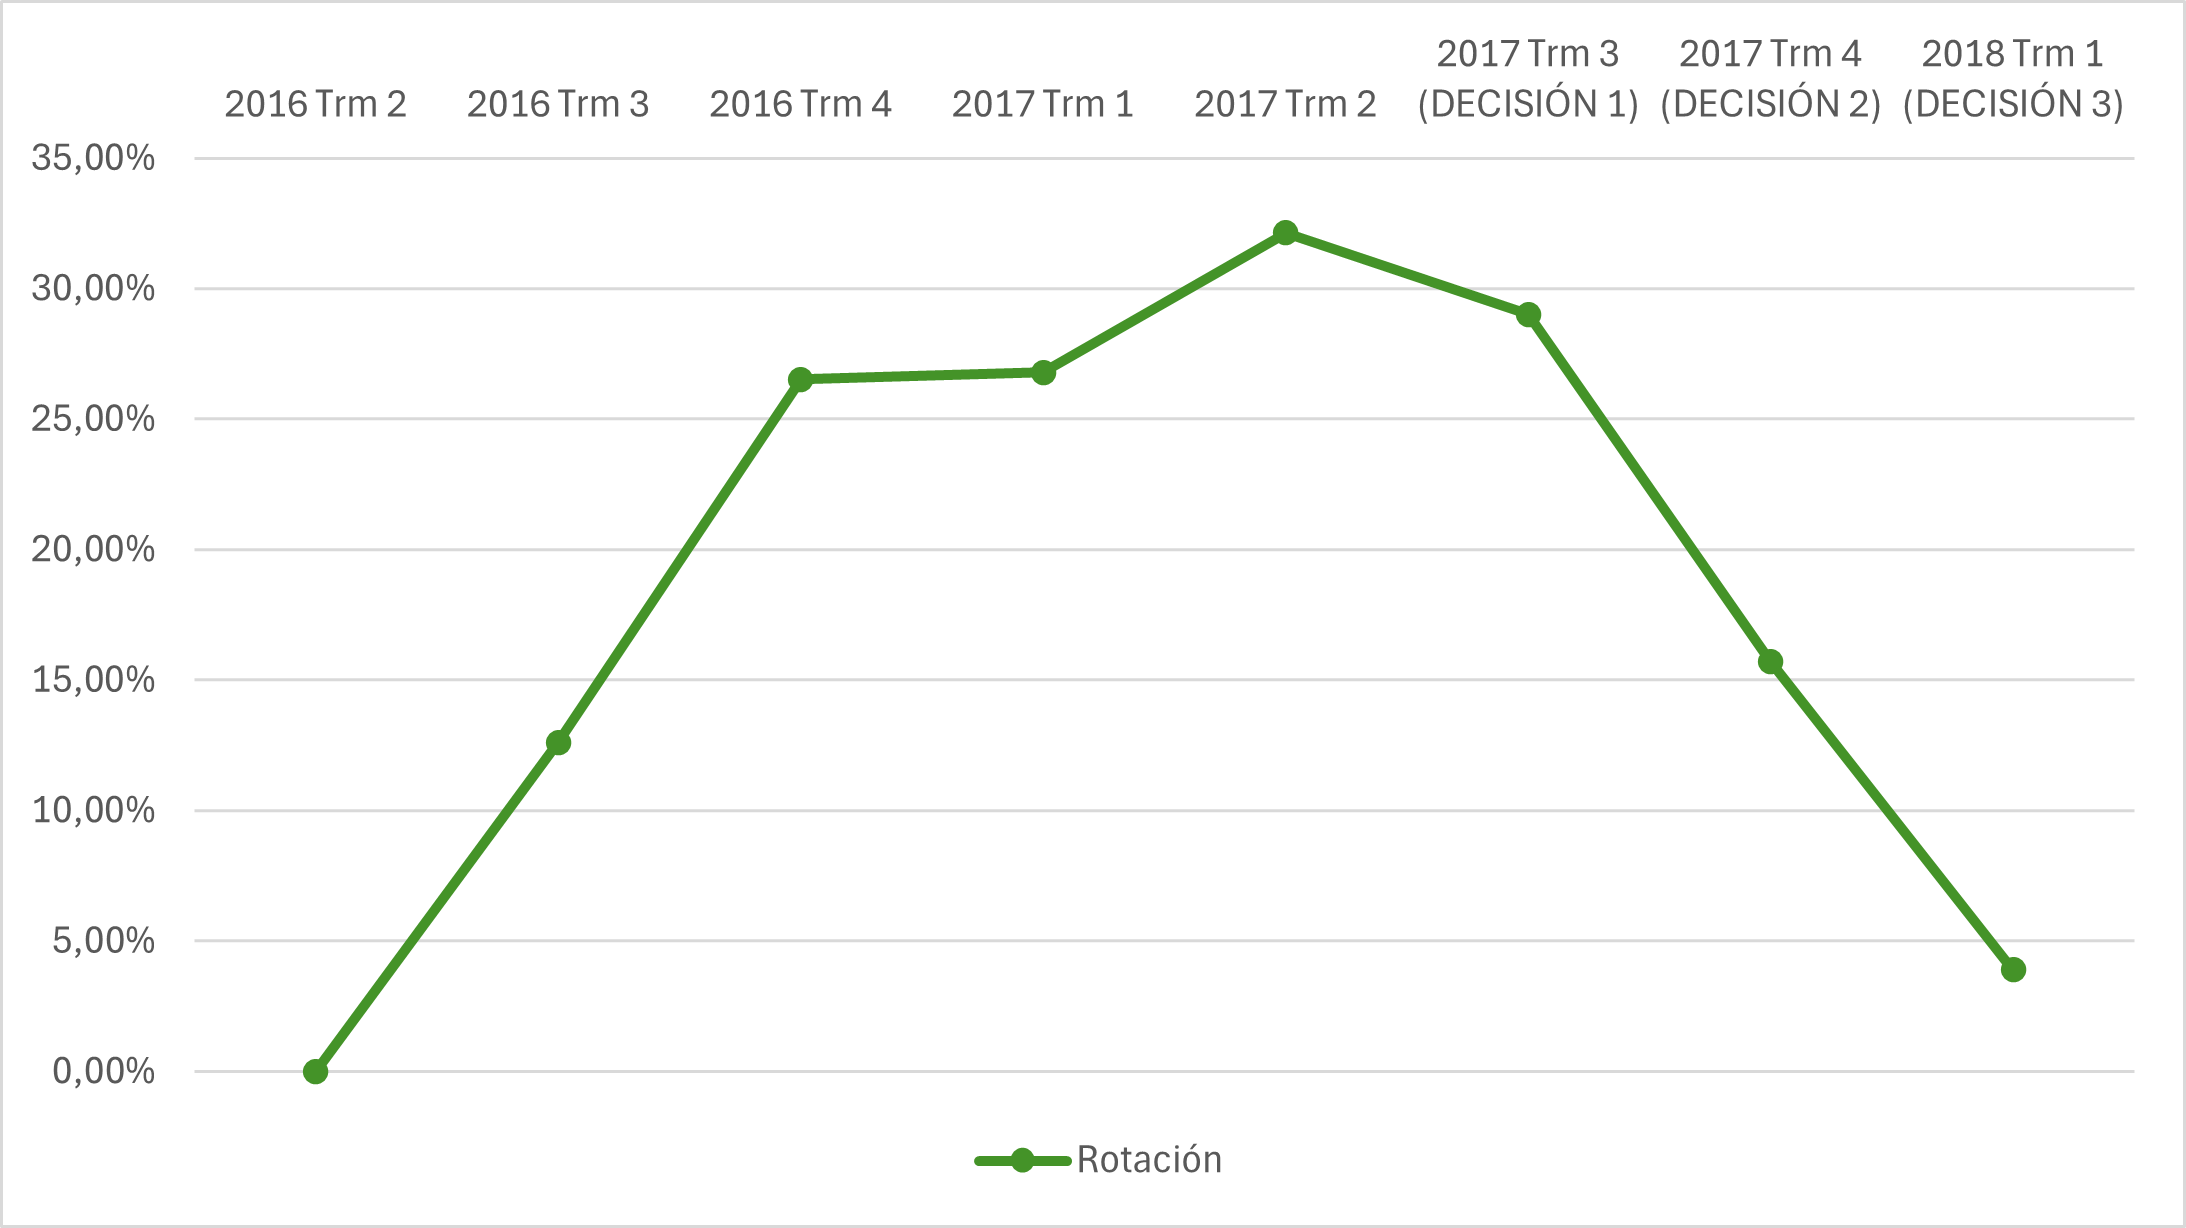
\includegraphics[width= \columnwidth]{Imagenes/decision3_rotacion activos.png}
\end{figure}

\section*{Publicidad para Estanterías Vacías}
En un intento por mantener la cuota de mercado, la empresa ejecutó una inversión agresiva en marketing, destinando partidas significativas a publicidad en Europa, Nafta e Internet, acompañadas de una política de precios premium. Sin embargo, los informes de ventas revelan grandes roturas de stock. La inversión publicitaria logró atraer a los clientes, pero la incapacidad logística para atender los pedidos convirtió ese gasto en una pérdida neta, dañando no solo la rentabilidad sino potencialmente la imagen de marca. 

Se produjo una diferencia notable entre lo invertido en la publicidad y lo obtenido en las ventas. Las ventas son un reflejo de los pedidos satisfechos, que son mucho menores a los pedidos que deberían corresponder a la cantidad de publicidad que se ha llevado a cabo. 

\begin{figure}[h]
  \centering
  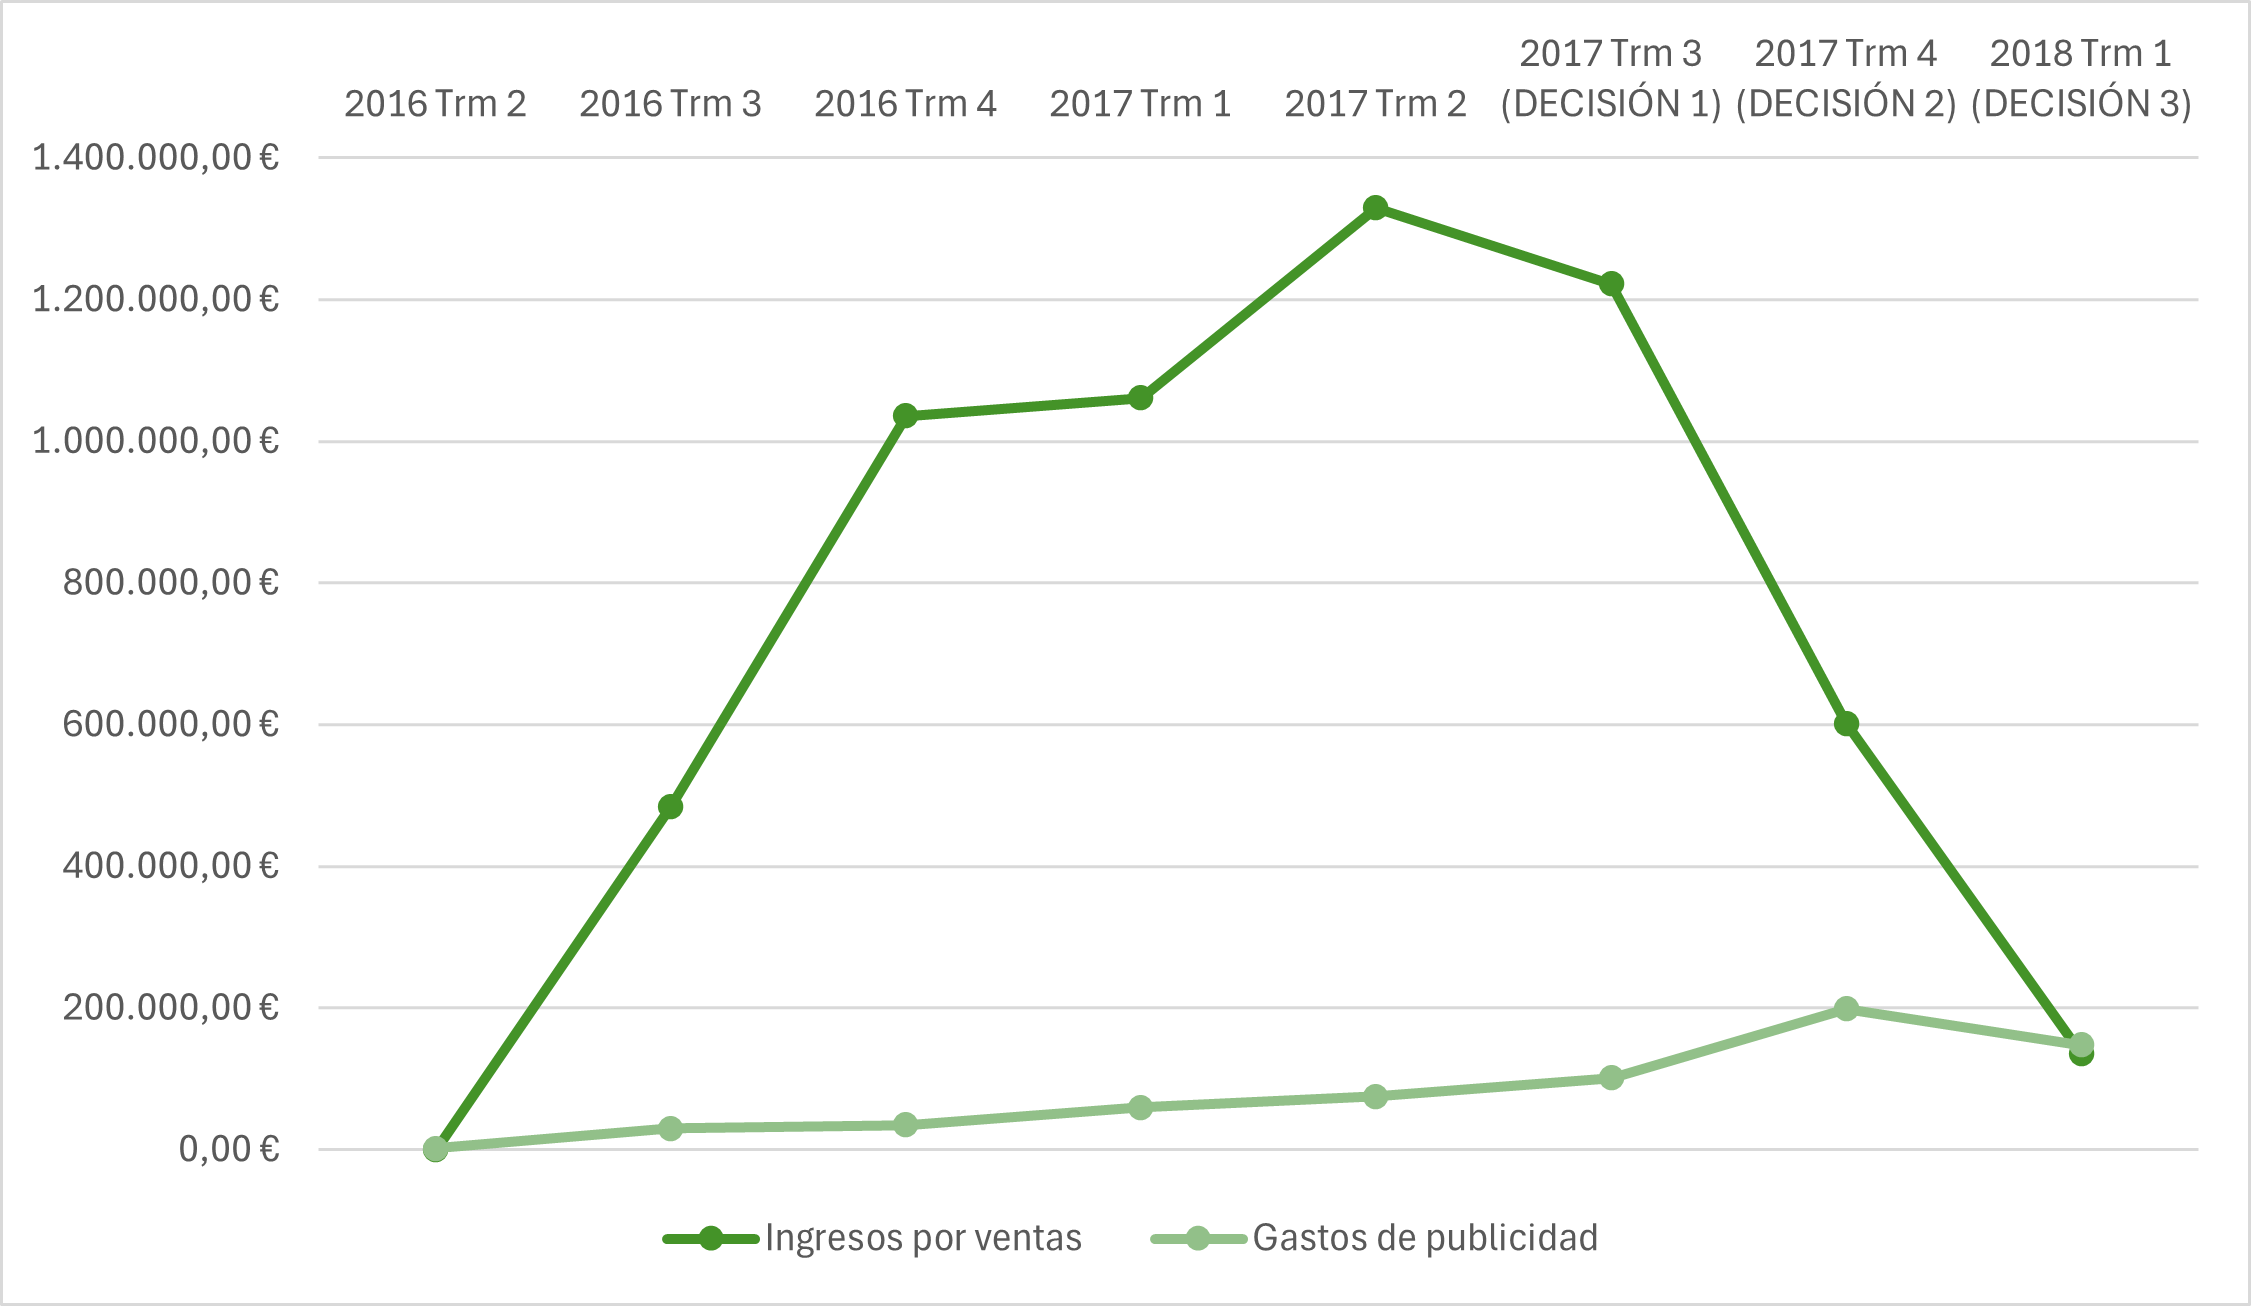
\includegraphics[width= \columnwidth]{Imagenes/decision3_ventas_publicidad.png}
\end{figure}

\section*{Números Rojos Históricos: La Estructura de Costes Devora la Caja}
La combinación de ventas mínimas y una estructura de costes fijos ha agujereado la cuenta de resultados. El trimestre cierra con unas pérdidas netas récord de 769.630 euros, una cifra alarmante que supera con creces cualquier beneficio obtenido anteriormente.  

El margen neto se ha desplomado hasta -566\%, lo que significa que, por cada euro facturado, la empresa ha perdido más de cinco euros debido al peso de los gastos operativos y estructurales que no pudieron ser absorbidos por el volumen de negocio. A esto afecta en gran medida el hecho de que las nuevas máquinas y los trabajadores, mantenidos en un sistema de doble turno, pasaran tiempo sin ser productivos. Los sueldos, el mantenimiento y la amortización de las nuevas inversiones se siguen pagando sin generar ningún beneficio, actuando como un drenaje constante del efectivo. Como respuesta la empresa tuvo que recurrir al préstamo para poder cubrir los costes fijos, en lugar de utilizar ese financiamiento para crecer. 

El análisis del beneficio bruto revela la envergadura de la crisis: el margen bruto fue de -248.554 €. Esto significa que el coste de producir y adquirir los bienes vendidos superó a los ingresos por ventas en 248.554 €. En términos porcentuales, esto representa un margen bruto negativo del -282.79\%. Este dato es demoledor.  

\begin{figure}[h]
  \centering
  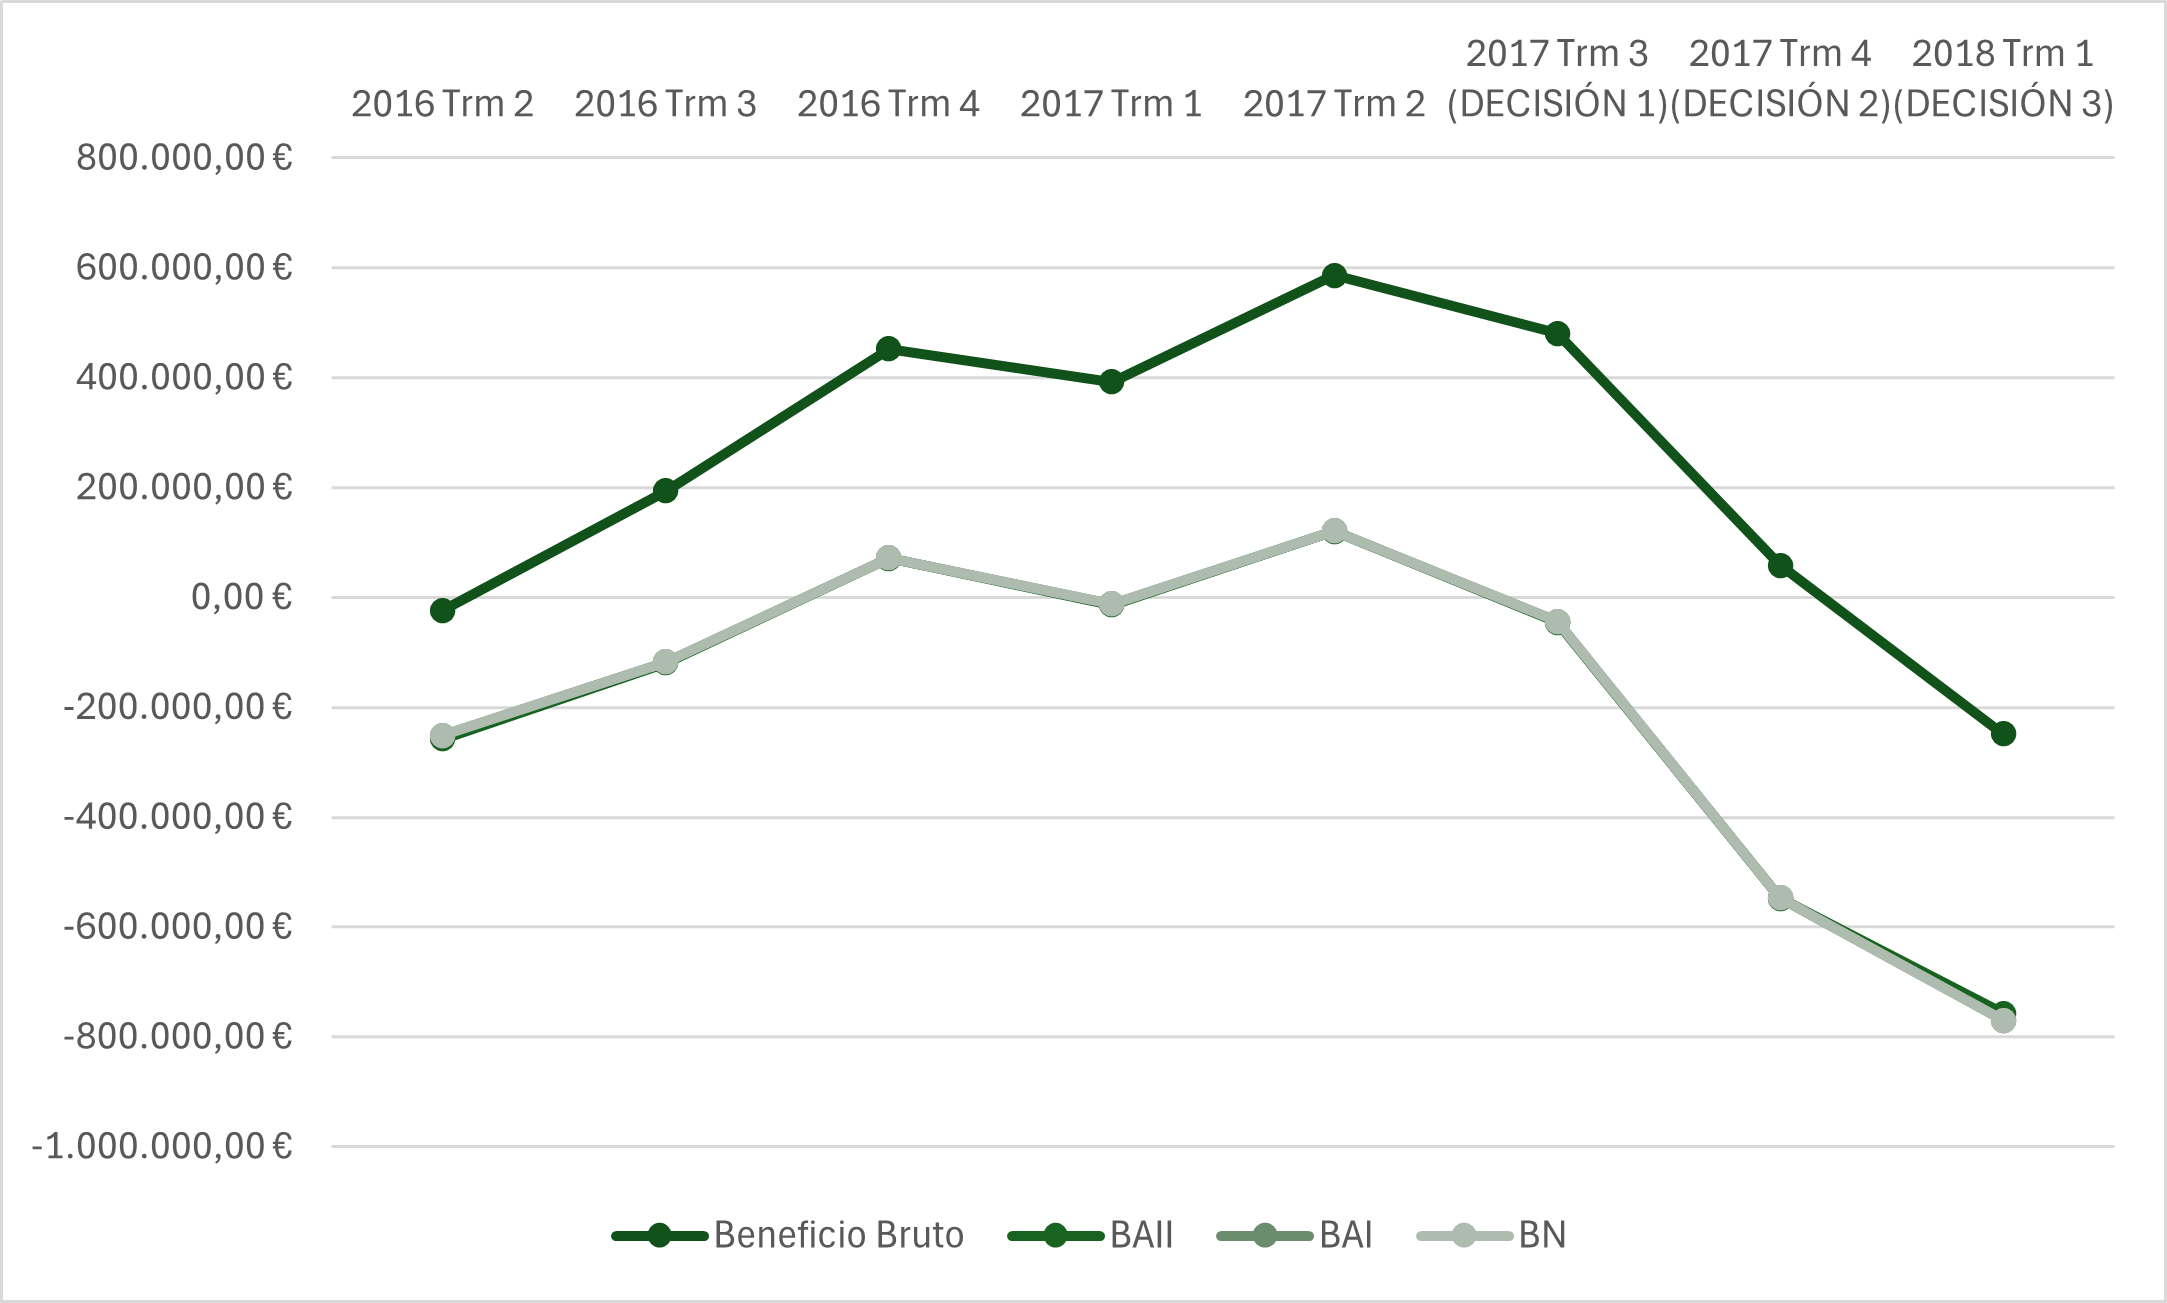
\includegraphics[width= \columnwidth]{Imagenes/decision3_beneficio bruto.png}
\end{figure}

\section*{Apuesta a la Desesperada: El Salto al 43\% de Apalancamiento en un Trimestre}
El pánico por la falta de liquidez y las pérdidas operativas forzó a la compañía a solicitar un préstamo a largo plazo de 500.000 € en este trimestre. Esta medida de emergencia elevó el pasivo de 606.061 € a 1.043.919 €, confirmando que el financiamiento externo se convirtió en la tabla de salvación ante el desastre operativo. 

Esta deuda no fue utilizada para generar ingresos o invertir en expansión productiva rentable, sino fundamentalmente para tapar el agujero de las pérdidas operativas (-769k €) y financiar la compra de maquinaria y ampliación de fábrica que, en ese momento, eran improductivas por falta de stock. 

Como resultado directo, el ratio de endeudamiento pasó de un 19\% en el trimestre anterior a un alarmante 43\% en un solo periodo. Este salto dramático indica que la empresa está asumiendo una carga financiera desproporcionada que será difícil de gestionar en los próximos trimestres, especialmente porque esta nueva deuda fue consumida sin generar un retorno inmediato. La tendencia ascendente del apalancamiento es un indicador de alto riesgo. 

\section*{Patrimonio en Peligro: Las Reservas Entran en Terreno Negativo}
El impacto acumulado de las pérdidas operativas ha causado un deterioro severo en el balance de la compañía. La cuenta de reservas se ha hundido hasta los -1.546.290 euros, lo que refleja que la empresa ha consumido gran parte de los beneficios históricos y del capital aportado para cubrir sus ineficiencias recientes. Como consecuencia directa, el patrimonio neto se ha reducido drásticamente, pasando de los 3,8 millones de euros a inicios del año anterior a 2.453.710 euros en la actualidad.  

Esta destrucción de valor se hace patente al analizar los indicadores de rentabilidad. La rentabilidad financiera (ROE) muestra un valor negativo de -31,37\%, lo que indica que, por cada 100 euros invertidos por los accionistas, se han perdido más de 31 euros en solo este periodo. La empresa vale hoy significativamente menos que al inicio de la simulación, y la capacidad de autofinanciación ha desaparecido por completo, dejando a la organización a merced de los acreedores externos. 

Finalmente, la comparativa entre la rentabilidad de los activos y la del accionista revela el efecto del endeudamiento. Mientras que la rentabilidad económica (ROA) se sitúa en un -21,65\%, el ROE cae aún más bajo (-31,37\%). Esta diferencia negativa demuestra que el apalancamiento financiero está actuando en contra de la empresa: al tener una rentabilidad de los activos muy inferior al coste de la deuda, el endeudamiento no hace más que amplificar las pérdidas para el accionista, acelerando la caída del patrimonio neto a una velocidad mayor que la caída de los activos. 

\begin{figure}[h]
  \centering
  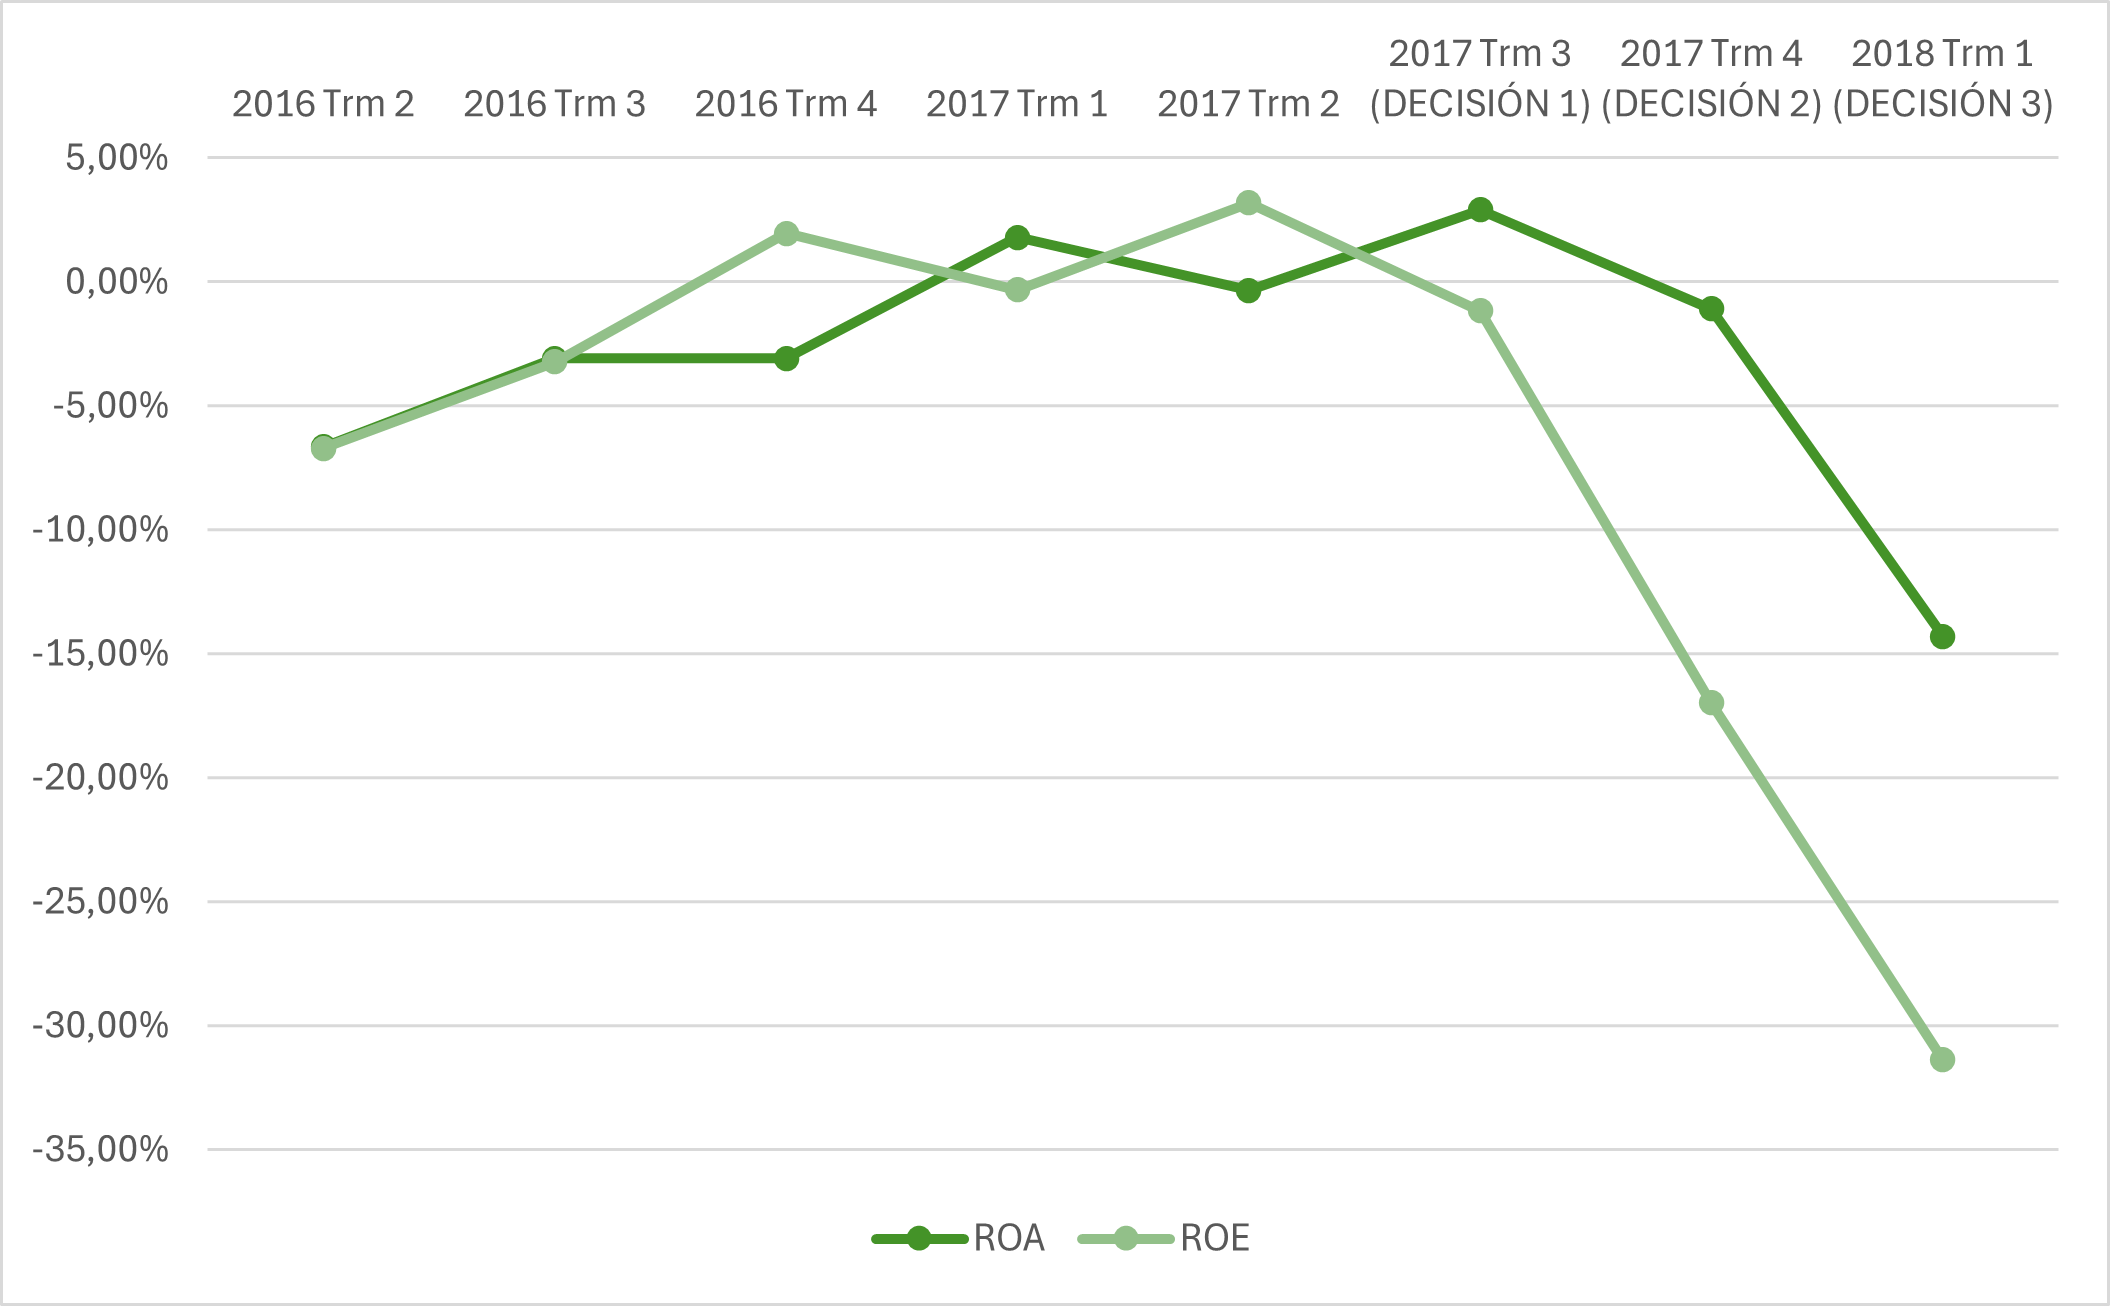
\includegraphics[width= \columnwidth]{Imagenes/decision3_ROA ROE.png}
\end{figure}

\section*{Lecciones Aprendidas y Lenta Recuperación}
Mirando hacia el futuro inmediato, la prioridad en los siguientes trimestres es corregir la falta de organización interna que paralizó la compañía. Ahora el objetivo debe centrarse en normalizar el suministro de materias primas para que la fuerza de ventas pueda capitalizar la demanda latente, con la esperanza de devolver la facturación a sus niveles históricos. 

Sin embargo, la dirección es consciente de que un simple aumento en las ventas no bastará para recuperar la caída de este trimestre. La empresa ha quedado financieramente debilitada, cargando ahora con una estructura de costes más pesada y una deuda creciente que exigirá recursos para su devolución. Por tanto, la recuperación no dependerá solo de vender más, sino de establecer una un sistema productivo de máxima eficiencia.  

\begin{table}[h]
    \centering
    \begin{tabular}{lr}
        \textbf{Balance - 3ª Decisión}               & \textbf{€} \\
        \hline
        \textbf{Activo fijo}                & \\
        Terreno                             & 50000 \\
        Bienes inmuebles                    & 262500 \\
        Valor de las máquinas               & 1577548 \\
        \cline{2-2}
        \textbf{Total activo fijo}          & \textbf{1890048} \\
        \textbf{Activo Circulante}          & \\
        Inventario - Productos              & 0 \\
        Inventario - Componentes            & 18700 \\
        Inventario - Materia Prima          & 1183207 \\
        Deudores                            & 110750 \\
        Efectivo e Inversores               & 294924 \\
        \cline{2-2}
        \textbf{Total activo circulante}    & \textbf{1607581} \\
        \cline{2-2}
        \textbf{Activo Total}               & \textbf{3497629} \\
        \textbf{Pasivo:}                    & \\
        Impuestos a pagar                   & 0 \\
        Acreedores                          & 543919 \\
        Línea de crédito / Descubierto      & 0 \\
        \cline{2-2}
        \textbf{Pasivo exigible}            & \textbf{543919} \\
        \textbf{Préstamos}                  & \textbf{500000} \\
        \textbf{Activo neto}                & \textbf{2453710} \\
        \textbf{Fondos propios}             & \\
        Capital social                      & 4000000 \\
        Prima de emisión                    & 0 \\
        Reservas                            & -1546290 \\
        \cline{2-2}
        \textbf{Patrimonio neto}            & 2453710 
    \end{tabular}
\end{table}

\begin{table}[h]
    \centering
    \begin{tabular}{|c|r|}
        \hline
        NOF & 1.063.662,00 € \\
        FM & -1.390.048,00 € \\
        EC & -2.453.710,00 € \\
        \hline
    \end{tabular}
\end{table}